\section{Il commence a faire chaud}

Date: 18/02/2008

\begin{multicols}{2}

Aujourd'hui, je vais vous livrer un petit secret : nos 3 phrases préférées du moment :
- "Dure la vie hein!", à prendre évidemment au second degré. On dort dans des hôtels sympa, on mange dans des restos très bons avec des vues exceptionnelles, le petit vent chaud du soir est très agréable, les palaces sont plus beaux les uns que les autres...
- "Ca fait combien de temps qu'on n'a pas vu un nuage?" La réponse commence à s'approcher gentiment de "deux semaines". Et oui, que du grand ciel bleu à l'horizon, du lever au coucher du soleil (qui sont toujours rouges, bleus, verts et violets on tient à préciser).
-"Ils sont fous, vraiment, complètement fous je te dis". Les Indiens bien sûre, on n'a pas idée de construire autant de merveilles au kilomètre carré. Les yeux grands ouverts on arrive toujours pas à tout capter ce qui se présente devant nous. Toutes les sculptures, tous les détails, le zèle des batisseurs... c'est incroyable.

Et au dela de ces impressions générales qui se confirment de jour en jour, nous continuons notre périple. Nous avons quitté notre hôtel ce matin à 5h, puis 3 grosses heures de bus pour arriver à Ranakpur. Là se trouve un des plus importants temples Jain de l'Inde, plus trois autres plus petits. Le gros comprends 29 pièces, et pas moins de 1444 colonnes de marbres sculptées (oui ils sont fous, on vous avait bien dit hein!). Les temples sont encastrés entre les montagnes, toutes recouvertes de verdure. On a même le plaisir de nourir les singes qui viennent calmement prendre des morceaux de gâteaux qu'on leur tend. Encore une halte fort agréable. Le soir, 4h30 de bus pour rejoindre Jodhpur où nous sommes actuellement. Ca semble promettre des moments sympa, surtout que nous allons y rester 5 ou 6 jours, jusqu'au moment de rentrer à Delhi pour faire des achats et prendre l'avion de retour. Et oui, on va être obligés de rentrer au bout d'un moment! En tout cas, on ne pense pas encore vraiment à ça et on profite à fond de chaque petit moment, de tout ce qui peut nous émerveiller : un oiseau vert et orange, des femmes rentrant des champs portant des fagots sur leur tête, des maisons de toutes les couleurs, les femmes qui lavent le linge sur les ghats... Nous passons tellement de moments intenses et indescriptibles! Le City Palace d'Udaipur qui s'illumine le soir, un spectacle de danse rajasthanie , la rencontre d'Indiens, mais aussi d'autres touristes, Européens, Américains ou encore Francais. On comprend de mieux en mieux l'anglais des Indiens et on relance les conversations. Nous croisons beaucoup de gens, mais brièvement. Nous nous fondons aussi de mieux en mieux dans le paysage, portant des habits plus "cool" et connaissant maintenant les combines des marchands. On ne prévoit plus ce qu'on fait, mais seulement on vit le moment à fond. Car l'Inde est un pays qui ne se raconte pas, mais qui se vit. Les photos sont peut-être jolies et les textes vous plaisent, mais tout ça n'est rien du tout par rapport à la réalité que nous vivons avec un grand plaisir chaque jour, chaque minute. Souvent les mots manquent pour exprimer ce que l'on ressent. On se contente alors d'un silence, d'un regard entre nous et d'un large sourire tout au fond du coeur. On ne réinventera pas les mots, nul besoin, car on sait très bien au fond de nous l'effet que ça produit, la trace que ça laissera, et c'est bien le principal.

\hspace*{-0.65cm}
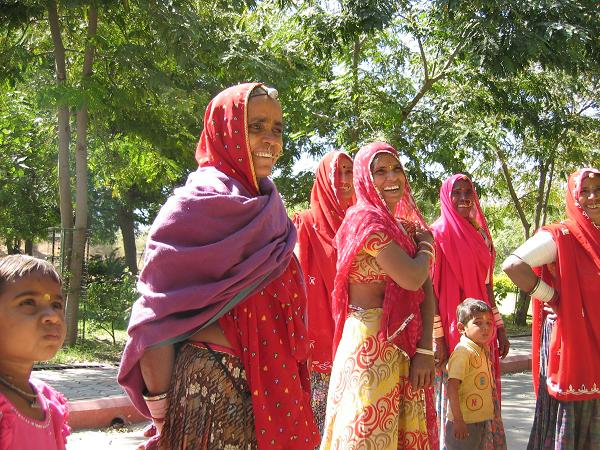
\includegraphics[width=4.8cm]{articles/Il-commence-a-faire-chaud/sari.jpg}
Des femmes en sari coloré

\hspace*{-0.65cm}
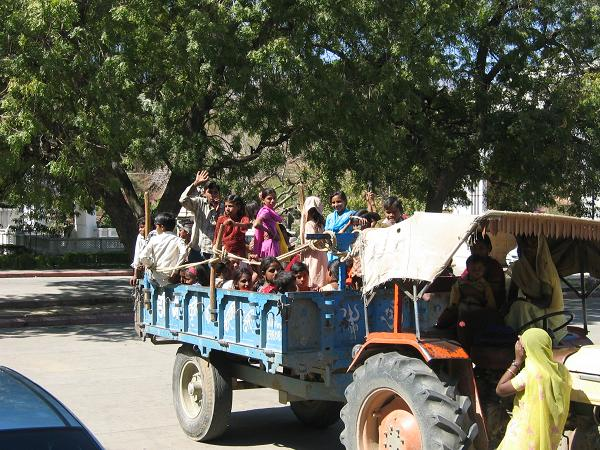
\includegraphics[width=4.8cm]{articles/Il-commence-a-faire-chaud/scolaire.jpg}
Un groupe d'enfants en sortie scolaire

\hspace*{-0.65cm}
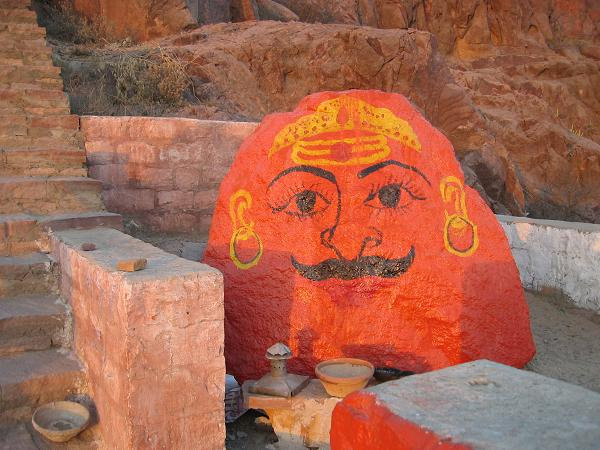
\includegraphics[width=4.8cm]{articles/Il-commence-a-faire-chaud/bonhommerouge.jpg}
Une icône peinte sur un rocher

\hspace*{-0.65cm}
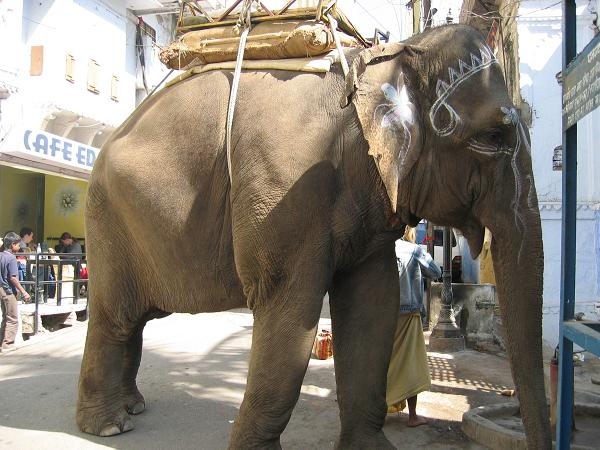
\includegraphics[width=4.8cm]{articles/Il-commence-a-faire-chaud/elephant.jpg}
Un éléphant dans une rue d'Udaipur

\hspace*{-0.65cm}
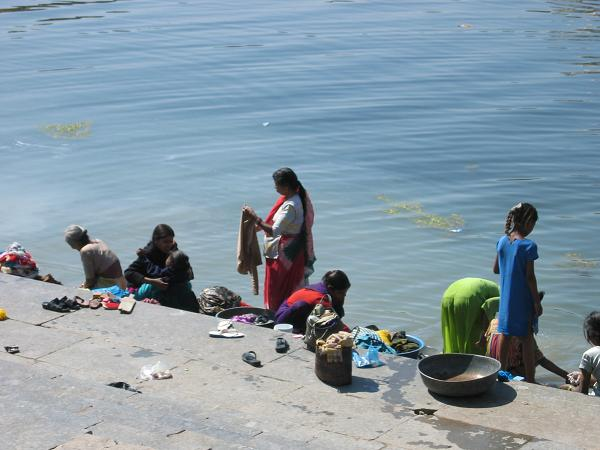
\includegraphics[width=4.8cm]{articles/Il-commence-a-faire-chaud/linge.jpg}
Des femmes lavant le linge sur les gaths

\hspace*{-0.65cm}
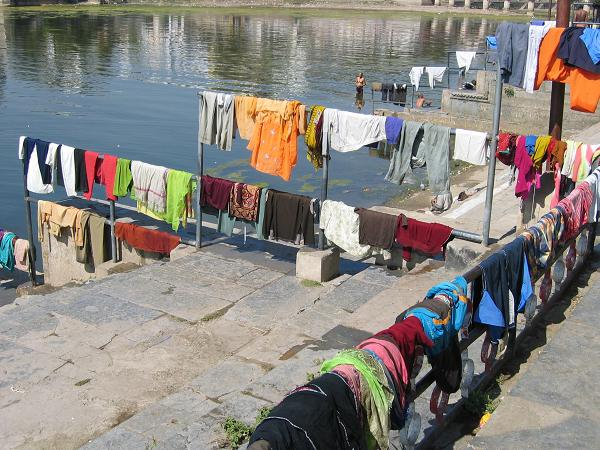
\includegraphics[width=4.8cm]{articles/Il-commence-a-faire-chaud/seche.jpg}
Le linge qui sèche

\hspace*{-0.65cm}
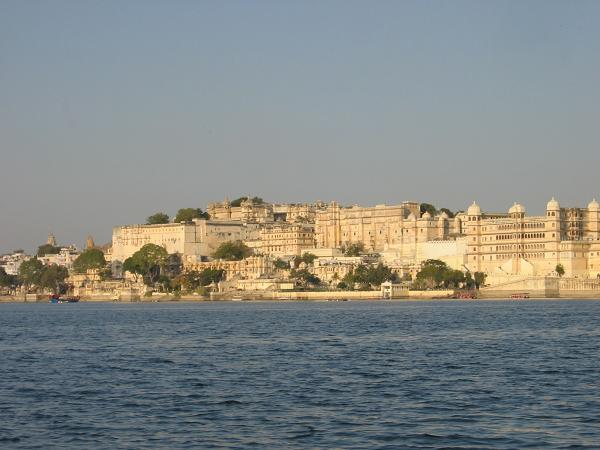
\includegraphics[width=4.8cm]{articles/Il-commence-a-faire-chaud/palacelac.jpg}
Le City Palace d'Udaipur vu depuis le lac

\hspace*{-0.65cm}
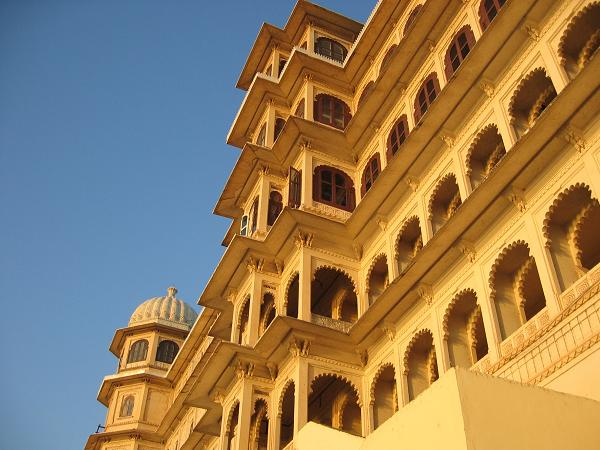
\includegraphics[width=4.8cm]{articles/Il-commence-a-faire-chaud/citylac2.jpg}
Une autre vue du City Palace

\hspace*{-0.65cm}
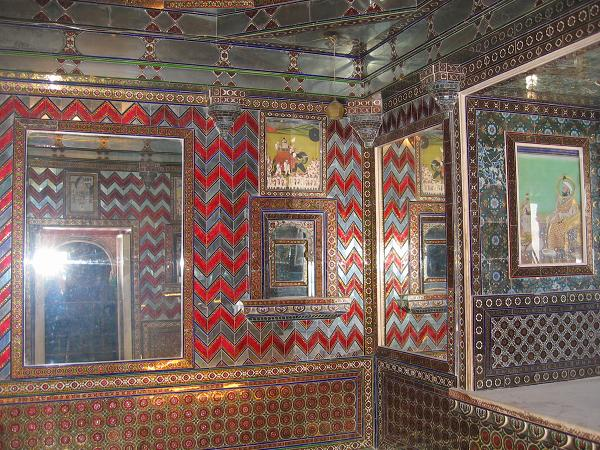
\includegraphics[width=4.8cm]{articles/Il-commence-a-faire-chaud/citysalle.jpg}
Une salle du City Palace

\hspace*{-0.65cm}
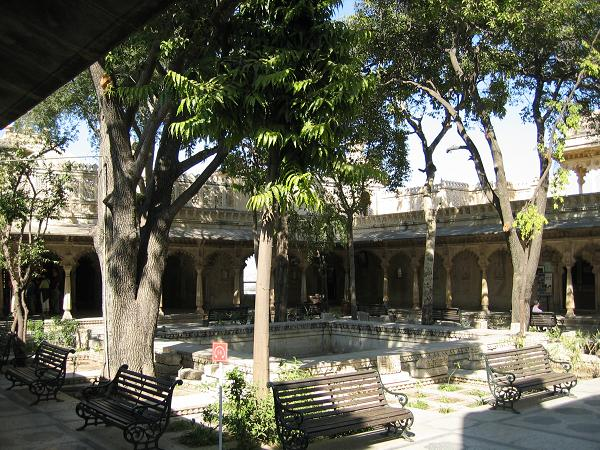
\includegraphics[width=4.8cm]{articles/Il-commence-a-faire-chaud/citycours.jpg}
Une cour intérieure

\hspace*{-0.65cm}
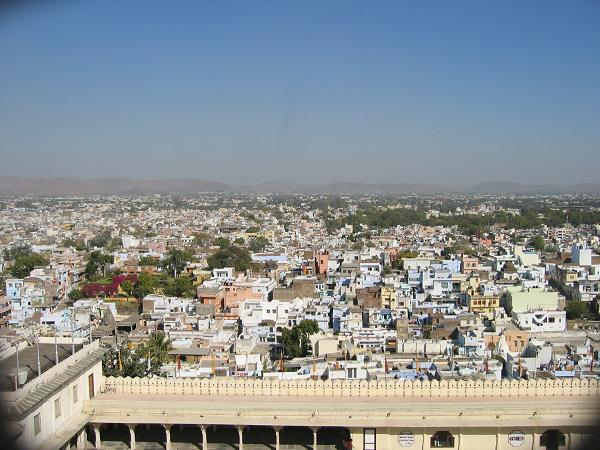
\includegraphics[width=4.8cm]{articles/Il-commence-a-faire-chaud/udaipur.jpg}
La ville d'Udaipur

\hspace*{-0.65cm}
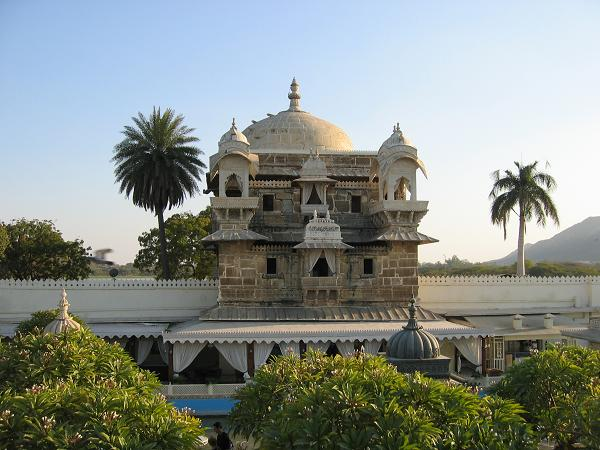
\includegraphics[width=4.8cm]{articles/Il-commence-a-faire-chaud/picchola.jpg}
Une belle vue depuis une île du lac Pichola

\hspace*{-0.65cm}
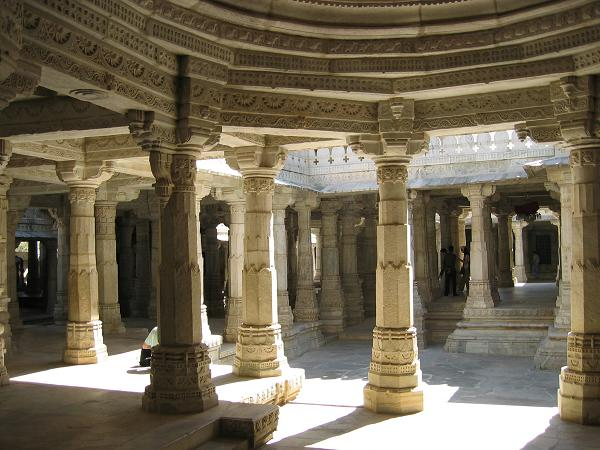
\includegraphics[width=4.8cm]{articles/Il-commence-a-faire-chaud/ranak.jpg}
Un immense temple Jain de Ranakpur

\hspace*{-0.65cm}
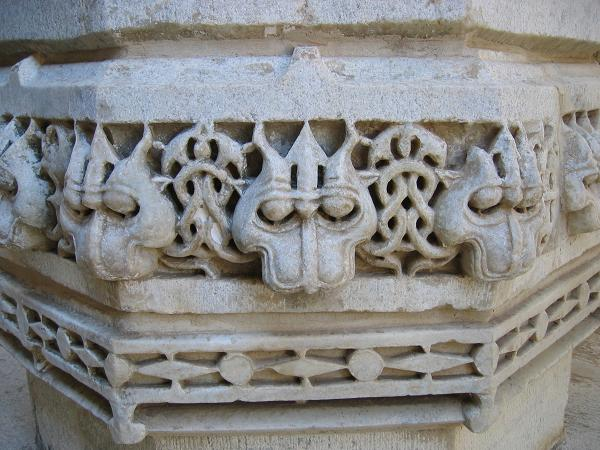
\includegraphics[width=4.8cm]{articles/Il-commence-a-faire-chaud/ranak2.jpg}
Le détail d'un temple

\hspace*{-0.65cm}
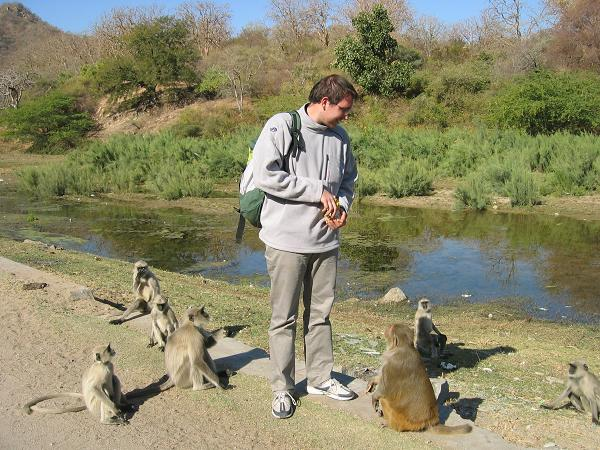
\includegraphics[width=4.8cm]{articles/Il-commence-a-faire-chaud/ranak3.jpg}
Etienne nourissant les singes

\hspace*{-0.65cm}
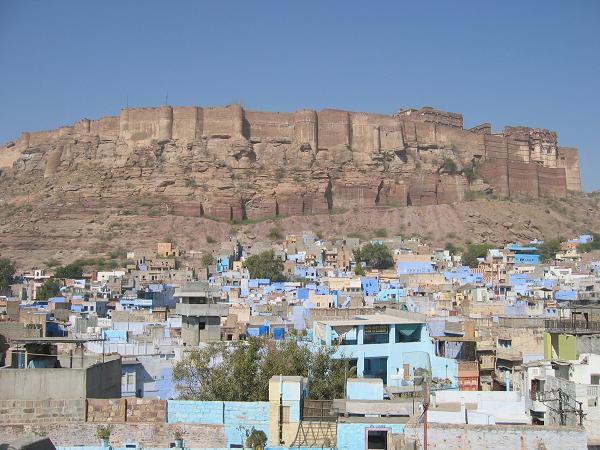
\includegraphics[width=4.8cm]{articles/Il-commence-a-faire-chaud/ranak4.jpg}
La vue depuis la terrasse de notre guest house de Jodhpur

Allez, parce que vous êtes sages, vous avez le droit à une video bonus

\end{multicols}
